%-------------------------------------------------------------------------------
%                             ADDITIONAL PACKAGES
%-------------------------------------------------------------------------------
\documentclass[
  letterpaper, 
%   showframes,
%   vline=2.2em,
  maincolor=black,
  sectioncolor=black!90,
  subsectioncolor=black!70,
  itemtextcolor=black!40,
%   sidebarwidth=0.4\paperwidth,
%   topbottommargin=0.03\paperheight,
%   leftrightmargin=20pt,
%   proilepicsize=4.5cm,
]{fortysecondscv}


\usepackage[T1]{fontenc}
\usepackage[utf8]{inputenc}


\usepackage[spanish]{babel}
\usepackage{graphicx}
\usepackage{fancyhdr}
\usepackage{blindtext}
\usepackage{geometry}
\usepackage{array}
\usepackage{multicol}
\usepackage{vwcol} 
\usepackage{tabulary}
\usepackage{url}
\usepackage{float}

% improve word spacing and hyphenation
\usepackage{microtype}
\usepackage{ragged2e}

% take care of proper font encoding
\ifxetexorluatex
	\usepackage{fontspec}
	\defaultfontfeatures{Ligatures=TeX}
% \newfontfamily\headingfont[Path = fonts/]{segoeuib.ttf} % local font
\else
	\usepackage[utf8]{inputenc}
	\usepackage[T1]{fontenc}
% \usepackage[sfdefault]{noto} % use noto google font
\fi

% enable mathematical syntax for some symbols like \varnothing
\usepackage{amssymb}

% bubble diagram configuration
\usepackage{smartdiagram}
\smartdiagramset{
  % defaut font size is \large, so adjust to harmonize with sidebar layout
  bubble center node font = \footnotesize,
  bubble node font = \footnotesize,
  % default: 4cm/2.5cm; make minimum diameter relative to sidebar size
  bubble center node size = 0.4\sidebartextwidth,
  bubble node size = 0.25\sidebartextwidth,
  distance center/other bubbles = 1.5em,
  % set center bubble color
  bubble center node color = maincolor!70,
  % define the list of colors usable in the diagram
  set color list = {maincolor!10, maincolor!40,
  maincolor!20, maincolor!60, maincolor!35},
  % sets the opacity at which the bubbles are shown
  bubble fill opacity = 0.8,
}


%-------------------------------------------------------------------------------
%                            PERSONAL INFORMATION
%-------------------------------------------------------------------------------
%%
%
% \cvprofilepic{img/logoUCR.png}

\cvname{\begin{center}
\includegraphics[width=0.5\textwidth]{img/logoUCR.png}
\\\vspace{-0mm}Universidad de\\Costa Rica\end{center}}

\cvjobtitle{\begin{center}
\includegraphics[width=0.5\textwidth]{img/logoEIE.png}\\\vspace{-0mm}Escuela de\\Ingeniería Eléctrica\end{center}}

%% optional information


% NOTE: ordering in sidebar will mimic the following order
% date of birth
% \cvbirthday{\textit{M. Sc.} Ricardo Román-Brenes}
% short address/location, use \newline if more than 1 line is required
% \cvaddress{\url{ricardo.roman@ucr.ac.cr}}
% phone number


%-------------------------------------------------------------------------------
%                              SIDEBAR 1st PAGE
%-------------------------------------------------------------------------------
% add more profile sections to sidebar on first page
\addtofrontsidebar{
	% include gosquare national flags from https://github.com/gosquared/flags;
	% naming according to ISO 3166-1 alpha-2 country codes

	% social network accounts incl. proper hyperlinks
	\profilesection{Estudiante}
		\begin{icontable}{2em}{1em}
		    % overleaf still not supports Academicons and FontAwesome5 for XeLaTeX, which contain the overleaf logl...unbelievable...
		    %\social{\aiOverleafSquare}
			\social{\faUser}
				{}
				{\textit{} Gabriel Araya Mora}
			\social{\faAt}
				{}
				{\url{gabomora2200@gmail.com}}
		\end{icontable}
		
	\profilesection{}
	 \tableofcontents
	 Glosario
	 
	 Proceso de instalación
	 
	 Especificaciones del computador
	 
	 Conclusión
       
    
}

\addtobacksidebar{
	% include gosquare national flags from https://github.com/gosquared/flags;
	% naming according to ISO 3166-1 alpha-2 country codes

	% social network accounts incl. proper hyperlinks
	\profilesection{Docente}
		\begin{icontable}{2.5em}{1em}
		    % overleaf still not supports Academicons and FontAwesome5 for XeLaTeX, which contain the overleaf logl...unbelievable...
		    %\social{\aiOverleafSquare}
			\social{\faUser}
				{}
				{\textit{M. Sc.} Ricardo Román-Brenes}
			\social{\faAt}
				{}
				{\url{ricardo.roman@ucr.ac.cr}}
		\end{icontable}
		
}


%-------------------------------------------------------------------------------
%                         TABLE ENTRIES RIGHT COLUMN
%-------------------------------------------------------------------------------
\begin{document}

\makefrontsidebar


\cvsection{\Huge \texttt{IE-0117} \textbf{Programacion bajo plataformas abiertas}}
\cvsubsection{\huge Laboratorio 0: Instalando GNU/Linux}
% \begin{cvtable}[1.5]
% 	\cvitem{2009 -- 2010}{Post-Doc Panda Studies}{Panda Academy}
% 		{In-depth studies on the impact of bamboo nutrition for young pandas and
% 		its relation to relaxing, sleeping and snoozing parts of the day.}
% 	\cvitem{2008 -- 2009}{Research Stay Europe}{European Panda Labs}
% 		{Spending one year abroad teaching european panda facilities about the
% 		newest findings and research in the field of asian rice hat covers and
% 		applications for bamboo as a material.}
% \end{cvtable}

% \cvsignature

\section{Glosario}
    \subsection{CPU:}
    Sigla de la expresión inglesa central processing unit, o por su traducción en español 'unidad central de                  				proceso', que es la parte de una computadora en la que se encuentran los elementos que sirven para procesar 						datos.
    
    \subsection{GPU:}
    GPU significa en inglés Graphics Processing Unit, en español Unidad de Procesamiento de Gráficos. El GPU es un 						chip procesador, como un chip CPU (Unidad Central de Procesamiento), pero es principalmente empleado para 							funciones gráficas en computadoras. Estas funciones gráficas pueden ser para efectos de luz, transformaciones de 				objetos, animación 3D, etc.
    \subsection{BIOS:}
    El BIOS (sigla en inglés de basic input/output system; en español "sistema básico de entrada y salida") es un 						software que localiza y reconoce todos los dispositivos necesarios para cargar el sistema operativo en la 							memoria RAM.
    \subsection{Kernel:}
    kernel es un software que constituye una parte fundamental del sistema operativo, y se define como la parte que 					se ejecuta en modo privilegiad. Es el principal responsable de facilitar a los distintos programas acceso seguro 				al hardware de la computadora o en forma básica, es el encargado de gestionar recursos, a través de servicios de 				llamada al sistema.
    \subsection{Partición de Disco:}
    Una partición de un disco duro es una división lógica en una unidad de almacenamiento.
\section{Instalación de GNU/Linux}
    El objetivo de este laboratorio es lograr instalar el sistema operativo Linux Mint 3 en uno de las sistemas de la universidad.Se empezó entrando al "boot louncher" de la computadora donde se le indicó al BIOs que debía iniciar desde el dispositivo USB, en el cual previamente se puso el ejecutable de Linux para ser instalado.
    
    
    Una vez que el Linux esta corriendo directamente en el USB es importante que se escoja una partición del disco del disco duro en la cual se instalará, ya que estas computadoras cuentan con aproximadamente siete u ocho. Se usó la partición número siete (SDA7). Esto es importante ya que el sistema operativo necesariamente debe estar alojado en alguna unidad de almacenamiento donde el controlador pueda tener acceso. 
    
    
    \begin{figure}
        \begin{center}
            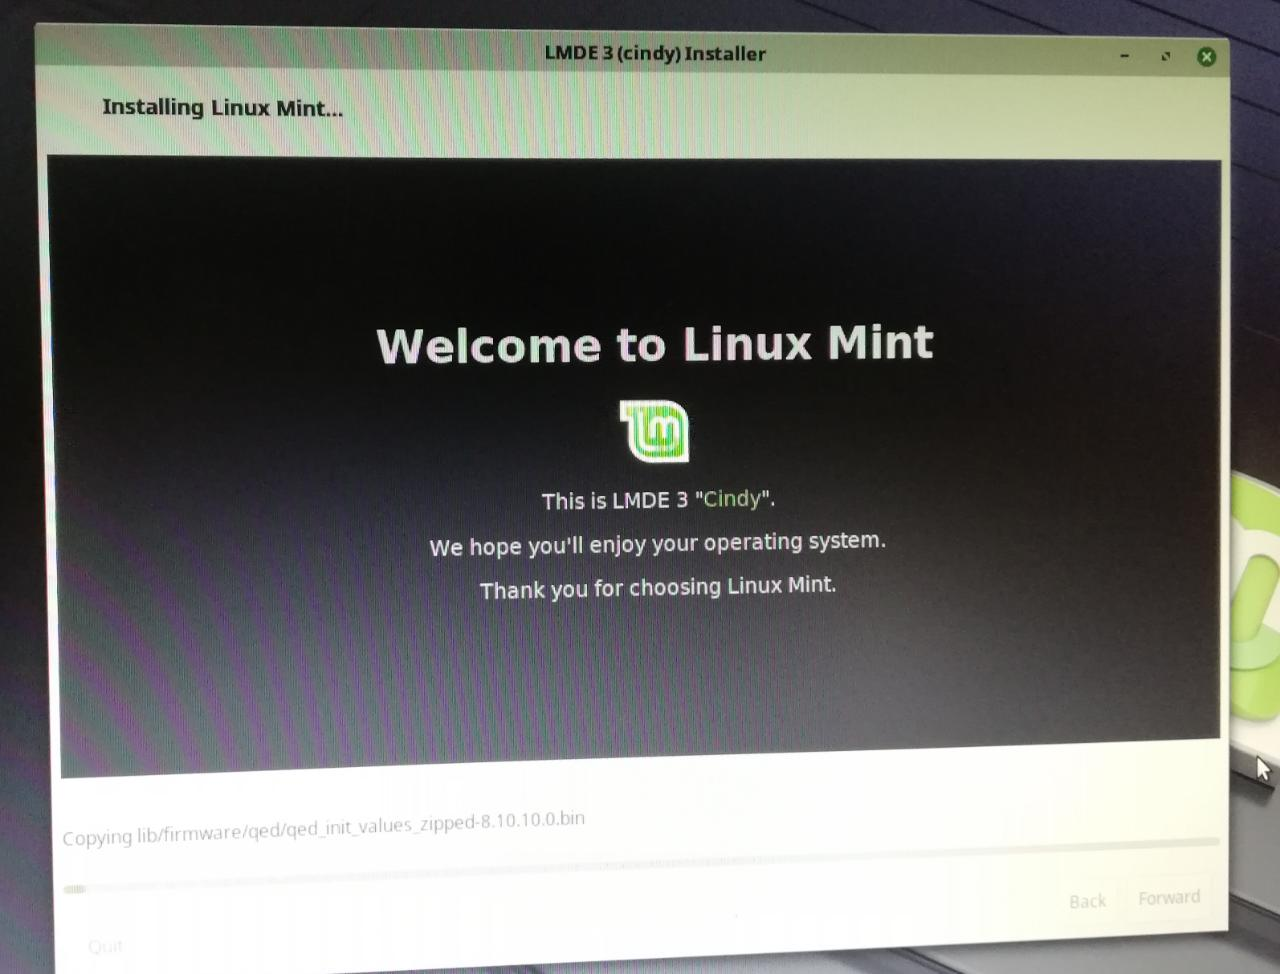
\includegraphics[width=6cm,lenght=5cm]{img/imagen1.jpg}    
        \end{center}
        \caption{Instalación Linux}
    \end{figure}
    
    
    Para finalizar la instalación del sistema operativo, se  debe crear un usuario, para esto el computador pide por entrada un nombre el cual se le dará al usuario y una contraseña. Es importante acomodar la zona horaria de la mejor manera ya que si no se hace, cualquier cosa que dependa de esto tendrá un desfase causando problemas a futuro.
    
    
    \begin{figure}
        \begin{center}
            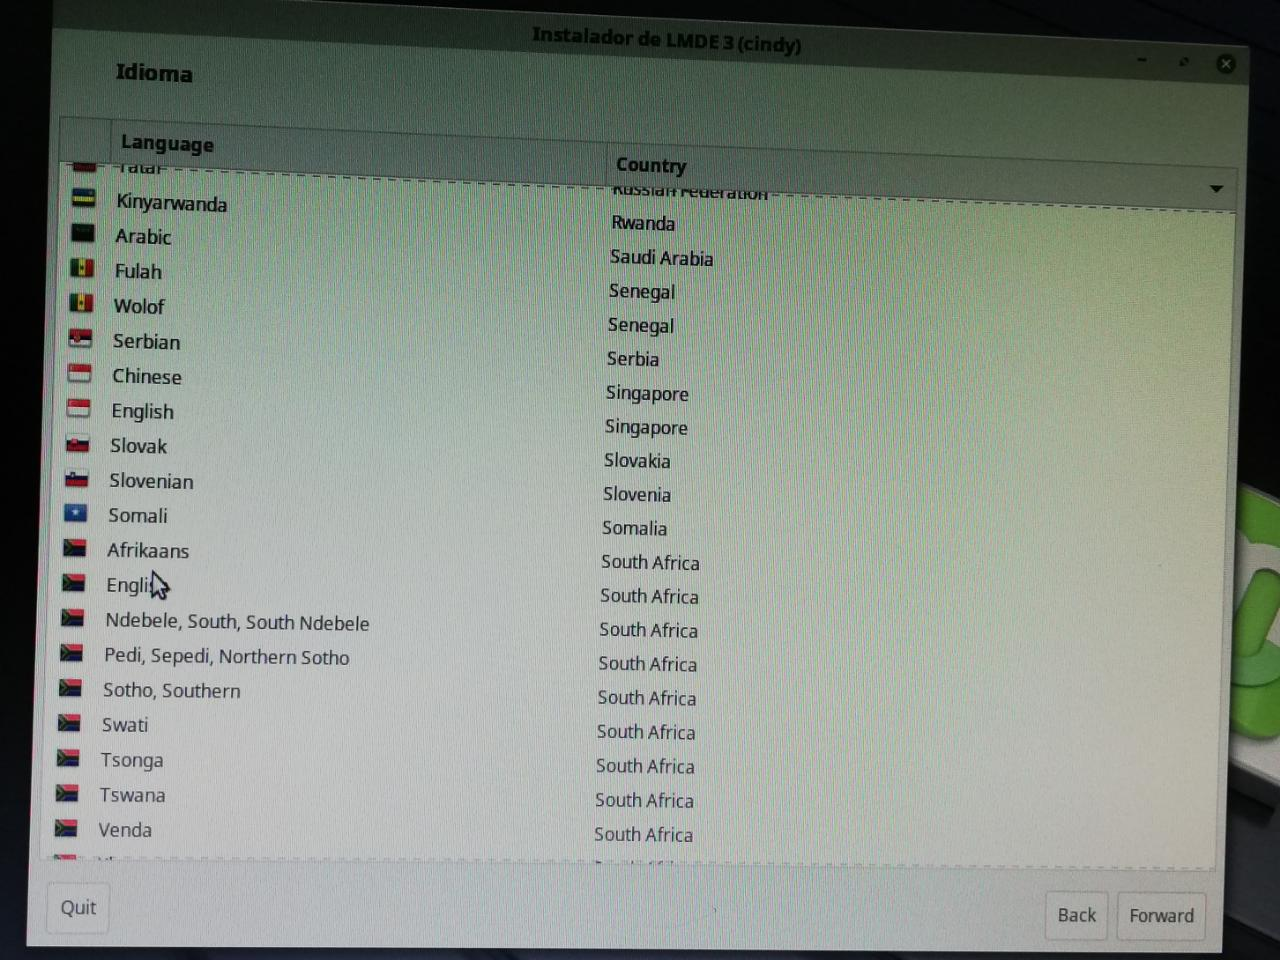
\includegraphics[width=6cm,lenght=5cm]{img/imagen2.jpg}    
        \end{center}
        \caption{Configuración de Linux}
    \end{figure}
    
    
    \begin{figure}
        \begin{center}
            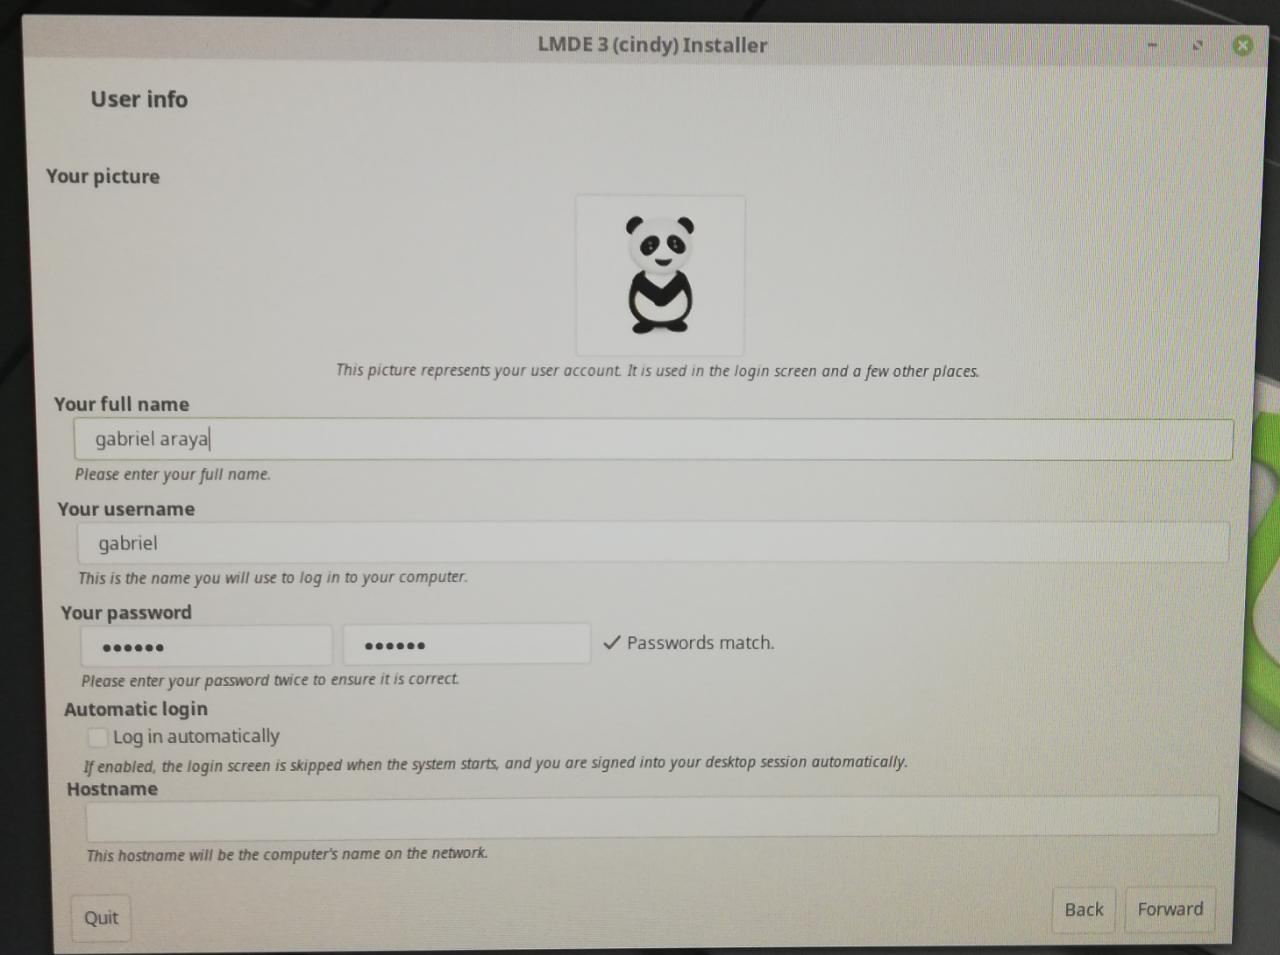
\includegraphics[width=6cm,lenght=5cm]{img/imagen3.jpg}    
        \end{center}
        \caption{Creación de Usuarios}
    \end{figure}
    
    \begin{figure}
        \begin{center}
            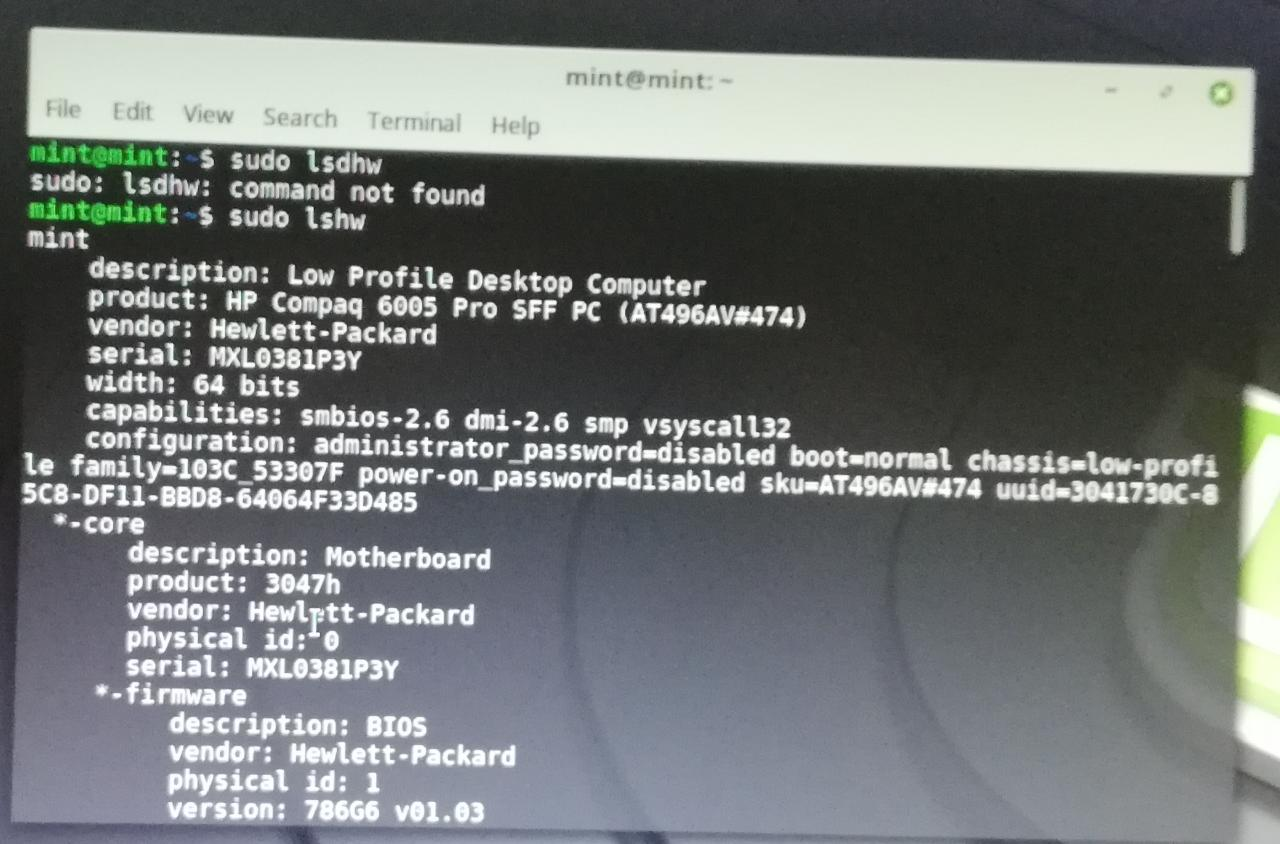
\includegraphics[width=6cm,lenght=5cm]{img/imagen4.jpg}    
        \end{center}
        \caption{Buscando especificaciones}
    \end{figure}

\newpage
    \section{Especificaciones del computador}
        \subsection{Modelo de CPU:}
            AMD Ahtlon II X2 B24
        \subsection{Frecuencia de CPU:}
            3.0 GHz
        \subsection{Cantidad de memoria RAM:}
            1.7 Gb
        \subsection{Espacio en el Disco duro:}
            50.1 Gb
        \subsection{Versión de Linux Mint:}
            LMDE 3 CINDY
        \subsection{Versión del Kernel de Linux:}
            4.9.0-7-AMD64
        
\section{Conclusión}
    En resumen se logró instalar de manera exitosa el sistema operativo en la partición indicada. Se eligió adecuadamente el nombre de usuario y la contraseña. Para encontrar las especificaciones del computador fue necesario usar el comando " sudo lshw ". El cual monstró en pantalla todos y cada uno de los componentes de la computadora, su fabricante y descripción. 
    
    


\end{document} 
